\documentclass[parskip=full]{scrartcl}
\usepackage[T1]{fontenc}
\usepackage[utf8]{inputenc}
\usepackage[ngerman]{babel}
\usepackage{hyperref}
\hypersetup{
	pdftitle={PSE: Blockchain-basiertes E-Voting - Implementierungsbericht},%
	,%
}
\usepackage{graphicx}
\usepackage{csquotes}
\usepackage[nonumberlist]{glossaries}
\usepackage{enumitem}
\usepackage{xcolor}
\usepackage{svg}
\usepackage[section]{placeins}

\makeatletter
\AtBeginDocument{%
	\expandafter\renewcommand\expandafter\subsection\expandafter{%
		\expandafter\@fb@secFB\subsection
	}%
}
\makeatother
\makeatletter
\AtBeginDocument{%
	\expandafter\renewcommand\expandafter\subsubsection\expandafter{%
		\expandafter\@fb@secFB\subsubsection
	}%
}
\makeatother

\addto\extrasngerman{\def\figureautorefname{Abb.}}
\newcommand{\textitx}[1]{\mbox{\textit{#1}}}
\newcommand{\fakeparagraph}[1]{\textbf{#1}}
%\renewcommand{\includesvg}[1][1]{}


\title{
	PSE:Blockchain-basiertes E-Voting \\
	Implementierungsbericht
}
\author{Tim Fröhlich, Achim Kriso, Philipp Schaback, David Schuldes, Artem Vasilev\\ Phasenverantwortlicher: Philipp Schaback}



\begin{document}
\clearpage
\maketitle
\pagenumbering{gobble}
\newpage

\tableofcontents
\newpage
\pagenumbering{arabic}

\section{Einleitung}
Dieses Dokument beschreibt die Ergebnisse der Implementierungsphase, die
im Rahmen des Moduls Praxis der Softwareentwicklung (PSE) am Lehrstuhl „Anwendungsorientierte formale Verifikation" von Prof. Dr. Beckert am Karlsruher Institut für
Technologie entstanden sind.
Implementiert wurde die im Pflichtenheft vorgegebene und in der Entwurfsphase entworfene Software "Blockchain-basiertes Evoting".


\section{Zeitablauf}
Um einen schnellen und erfolgreichen Abschluss der Implementierung zu begünstigen, begann diese bereits Ende Juni.
Die im Entwurfsdokument angegebene Zeiteinschätzung wurde hierbei weitestgehend eingehalten, in vorteilhaft gestauchter Version (siehe \autoref{fig:gantt}).
\begin{figure}[h!]
	\centering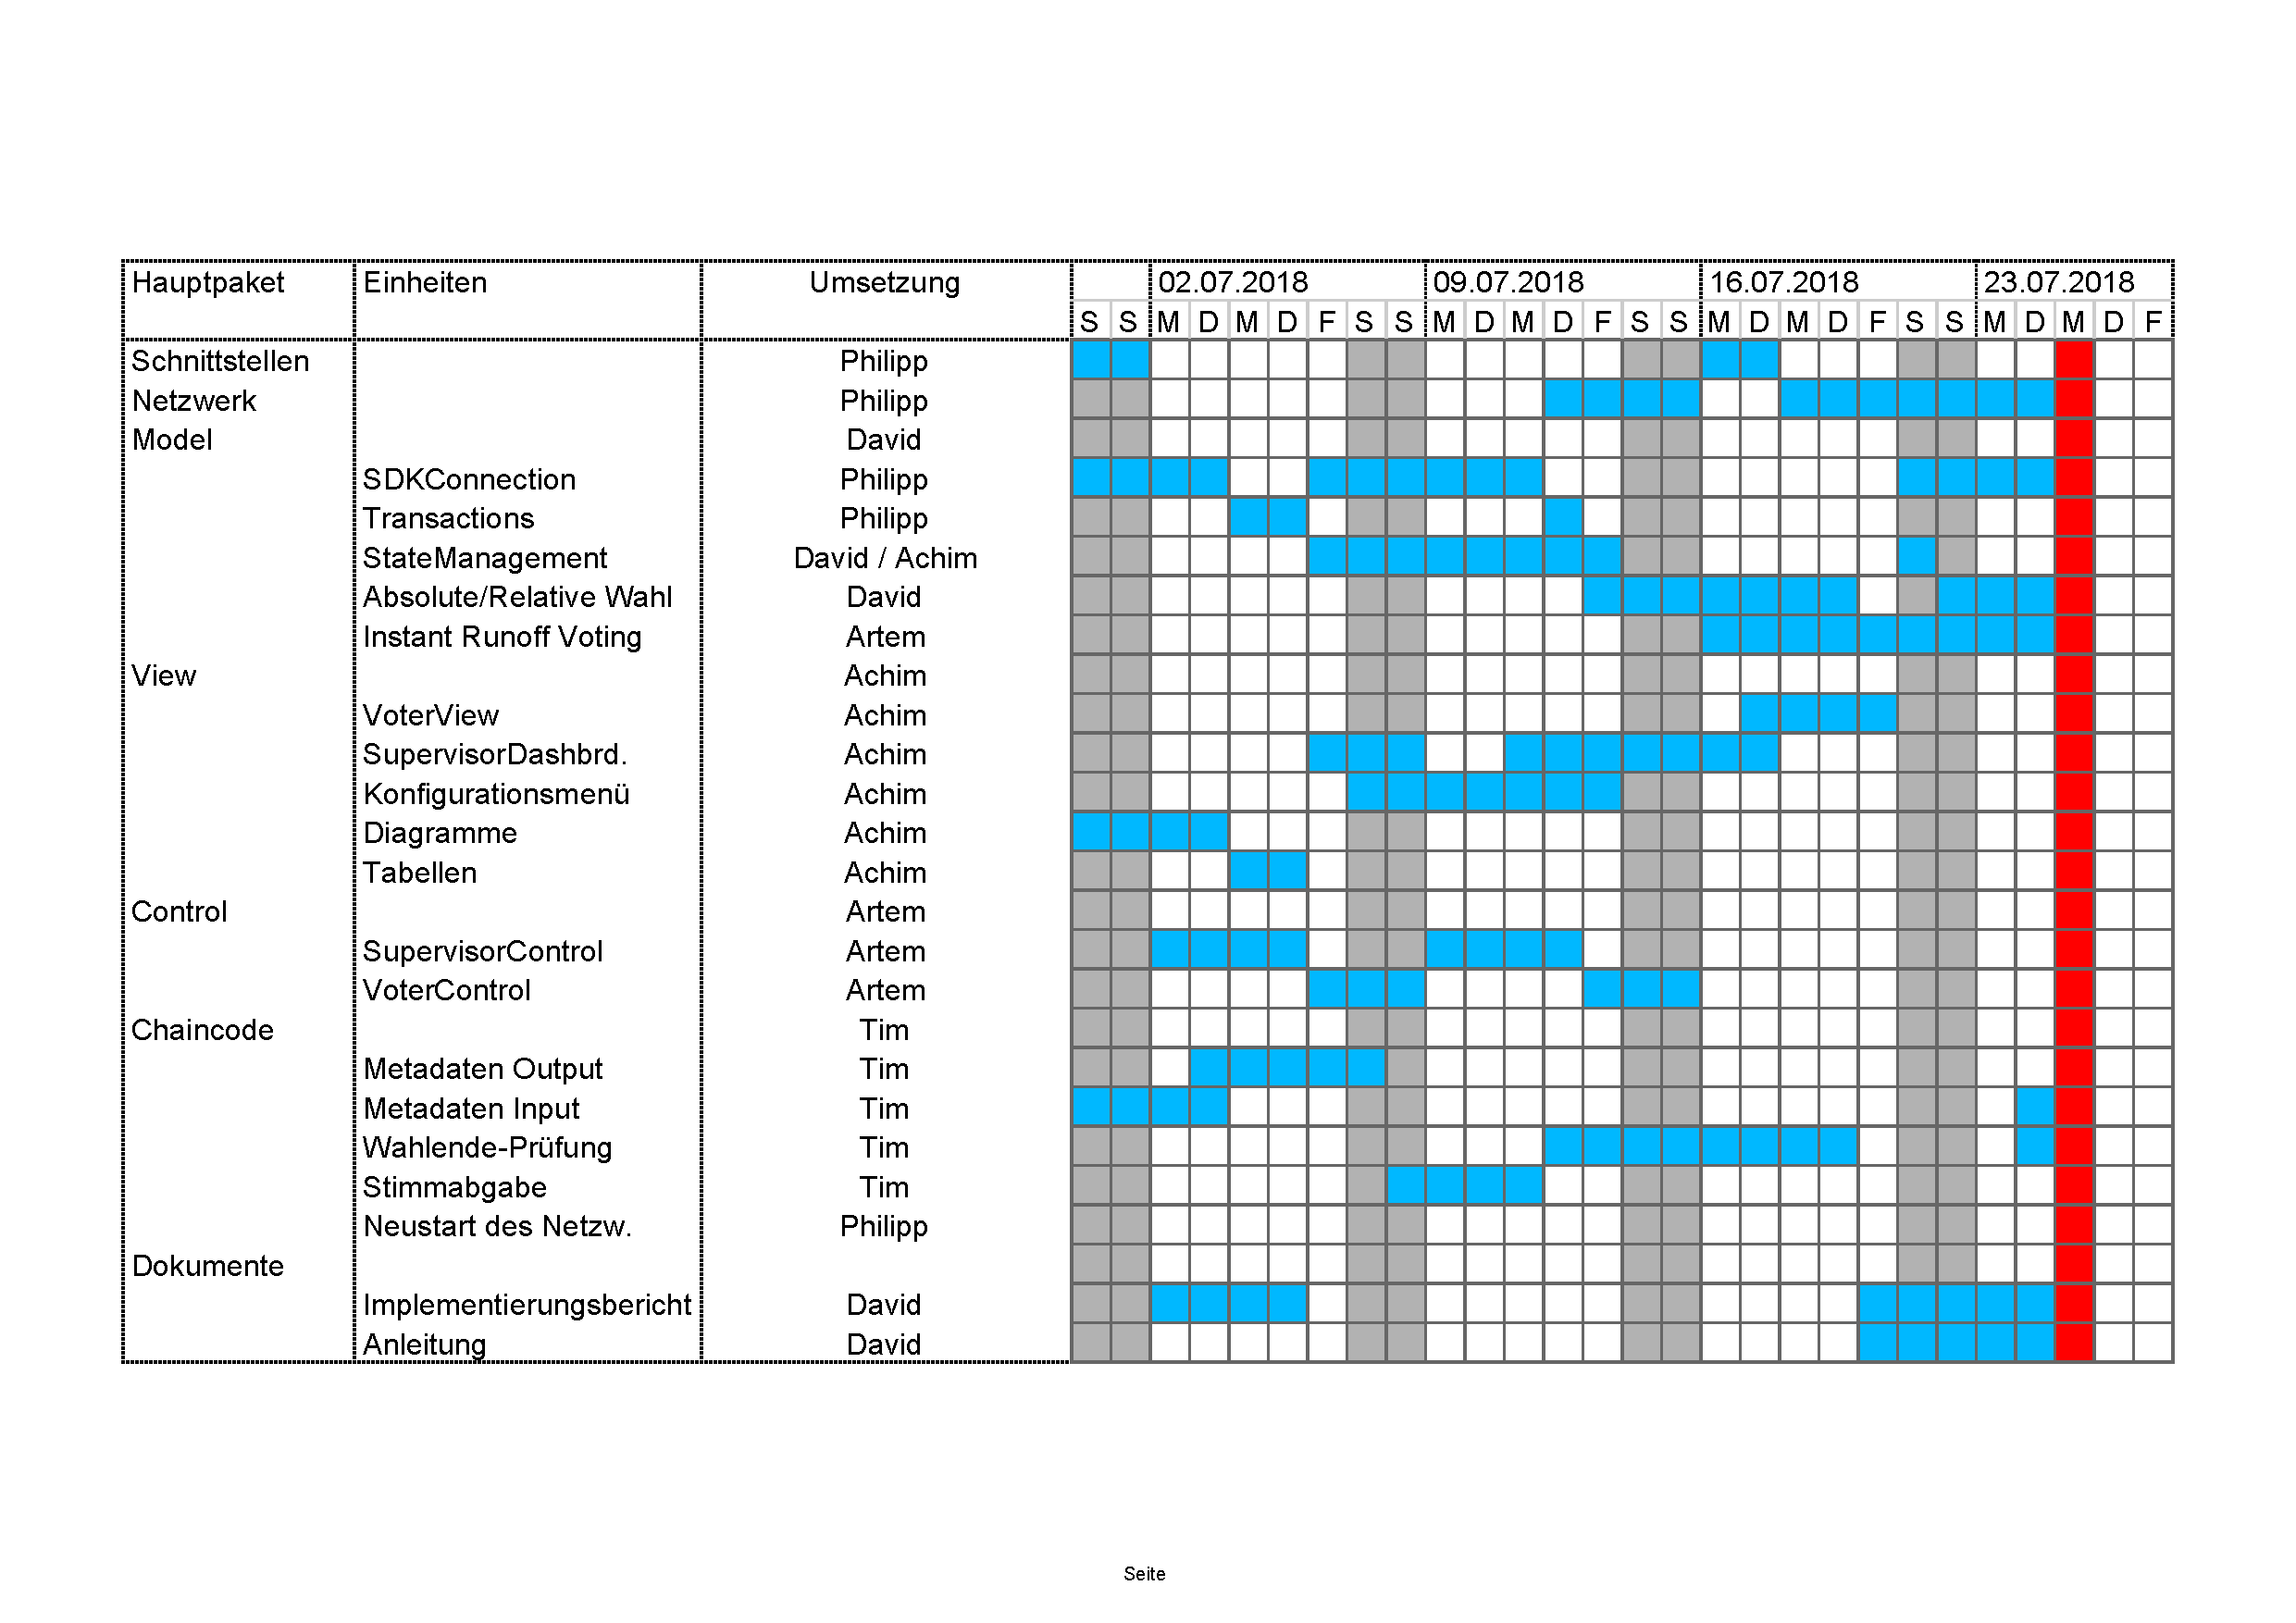
\includegraphics[width=\textwidth]{pictures/Gantt.pdf}
	\caption{Gantt-Diagramm (unvollständig)}
	\label{fig:gantt}
\end{figure}


\section{Umsetzung der funktionalen Anforderungen}

\subsection{Musskriterien}
Alle im Pflichtenheft festgelegten Musskriterien wurden durch die Implementierung umgesetzt.

\subsection{Sollkriterien}
Die Sollkriterien wurden alle bis auf eines erfüllt:
\textit{S3: Dynamische Peerverbindung}\\
Teil des Sicherheitsmodells von Hyperledger Fabric ist, dass ein Client Verbindungen zu mehreren Peers herstellt, das Kriterium sieht aber nur die Verbindung zu einem Peer vor.
Somit wäre eine Umsetzung von S3 der korrekten und sicheren Wahl entgegenstehend. Dennoch ermöglichen wir es, einzelne Peers mittels der Konfigurationsdate auszuschließen.  

\subsection{Kannkriterien}
Alle Kannkriterien, ausgenommen von \textit{K2: Geheime Wahlen} wurden umgesetzt. K2 wurde, wie schon im Entwurfsdokument begründet, nicht implementiert.

\section{Umsetzung der nichtfunktionalen-Anforderungen}

Alle im Pflichtenheft definierten, nicht-funktionale Anforderung wurden erfüllt. Im Folgenden sind sie in die Kategorien Zeitverhalten und Benutzerfreundlichkeit unterteilt.

\subsection{Zeitverhalten}

\begin{itemize}
	\item Die Stimmabgabe eines Wählers dauert vorraussichtlich nicht länger als 5 Minuten.
	\item Die grafische Benutzeroberfläche reagiert sofort entsprechend der Aktion des Benutzers.
	\item Die Auswertung einer Wahl nimmt bei höchstens 10000 abgegebenen Stimmen vorraussichtlich nicht mehr als 5 Minuten in Anspruch.
\end{itemize}

\subsection{Benutzerfreundlichkeit}
\begin{itemize}
	\item Die Benutzung der Software erfordert keine besonderen Vorkenntnisse, so dass sie auch Benutzer mit geringen Computerkenntnissen verwenden können.
\end{itemize}

\section{Produktleistungen}
Erfolgreich abgegebene Stimmen gehen unverfälscht in die Auswertung der Wahl ein und werden genau einmal gewertet. Es ist nicht möglich, Stimmabgaben zu verfälschen und somit das Ergebnis der Wahlauswertung zu manipulieren.
		
\section{Umsetzung von Entwurfsentscheidungen}


\section{Änderungen zum Entwurf}


\end{document}

